% !TEX root = ../main.tex

\section{Ablating \isklearn}
\label{sec:further}

Results from the first part of our investigation validated our \irace AutoML proposal as a competitive approach in terms of efficacy. We next ablate \isklearn to understand how the proposed configuration space and setup affect its performance. We start with a configuration space analysis,  where we assess the benefits of having a minimalist template. Later, we appraise different configuration setups, exploring the idea of the generalized mid-level sampling and providing guidelines for the application of \isklearn to other problems.

% Yet, CIFAR-10 results indicate that further investigation is required on more challenging domains, such as computer vision. In this section, we assess~(i)~alternative configuration setups and~(ii)~the feasibility of transfer learning. The datasets adopted in this section were chosen for their popularity in the small image classification literature. Specifically, we replace MNIST with Fashion MNIST~(FMNIST), given the small margin for improvement on the former. In addition, we also consider CIFAR-100, a dataset similar to CIFAR-10, and SVHN, a house number recognition problem. Further information on these datasets is given in the supplementary material, particularly the details on manual data preparation, sampling, and resource limits for \autosklearn.

%\input{sections/transfer-learning}
\subsection{Comparing Configuration Spaces}

To assess the benefits of having a simpler template in terms of efficacy of the pipelines produced, we use SMAC~\cite{smac} to configure pipelines from our template. Since SMAC is the configurator powering \autosklearn, the comparison given in Figure~\ref{fig:smac} helps us isolate the effects of configurator and templated adopted. We focus this investigation on CV datasets as they were the most challenging for both AutoML approaches.

\begin{figure}
    \centering
    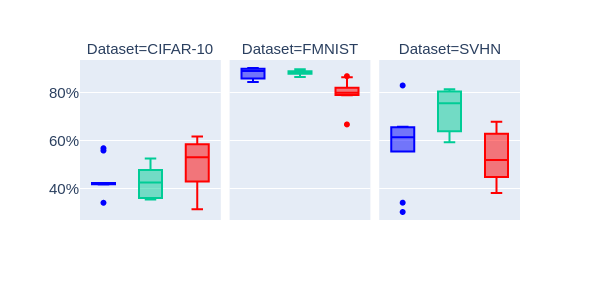
\includegraphics[width=\linewidth, clip=true, trim=45px 80px 80px 40px]{img/smac.png}
    \caption{Accuracy comparison between pipelines configured by \tinyirace~(blue) and SMAC~(green) from \tinyisklearn and ensembles configured by SMAC from \autosklearn~(red).}
    \label{fig:smac}
\end{figure}

Boxplots for the different datasets indicate that the performance of pipelines configured from \isklearn by SMAC are more similar in performance to pipelines configured from \isklearn by \irace than to the ensembles configured from \autosklearn by SMAC itself. 
% Interestingly, the distributions of the accuracy scores for the pipelines configured by SMAC and \irace are very different, with quartiles for \irace being located closer to their median than for SMAC, but presenting strong outliers. 
More repetitions of these experiments would be required to understand if the differences in distributions between \irace and SMAC results are consistent, or if the outliers observed are fluctuations in the experiments. Nonetheless, the comparison between pipelines and ensembles confirms that our proposed minimalist template is a contribution not only in terms of simplicity and interpretability, but also as to efficacy. Furthermore, it evidences the generality of the configuration space and setup proposed, as they can be coupled with any configurator that supports numerical, categorical, and conditional parameters, such as SMAC.

% !TEX root = ../main.tex

\subsection{Alternative Configuration Setups}
\label{sec:alt-setups}

Results discussed in Section~\ref{sec:results} indicated the efficacy of the configuration setup adopted, but some relevant questions need to be further investigated. We start with the analysis of the TS datasets. Our goal is to understand the impact of the different sampling generalization approaches we propose, in particular the bottom-level sampling cross-validation approach that should suit TS problems better than the traditional holdout.
Figure~\ref{fig:ts-setups} gives boxplots of experiments where we compare the original setup adopted in Section~\ref{sec:results}~(dubbed \textbf{regular}) and a setup where we increase the number of meta-folds to $p=3$ and total cutoff time to 15min~(dubbed~\textbf{TM}, for \textit{triple meta-fold}). For brevity, a discussion on the balance between the number of meta-folds and total cutoff time is provided as supplementary material.
% ADD TO SUPP!
%This change in setup aims to provide more samples to the bottom-level sampling, and thus reduce the chance of overfitting. However, having three times more samples incurs in a cutoff time issue for the evaluation of the meta-folds. On one hand, reusing the 10min total cutoff time from \textit{regular} would mean the cutoff time per meta-fold would be reduced to roughly 3min. On the other hand, preserving the cutoff time per metafold at 10min would increase the total cutoff time to 30min. In this initial experiments, we adopt a middle ground solution and set total cutoff time to 15min, which translates into 5min per-meta-fold cutoff time.
%
%where we reduce the number of setups considered, but include ensembles produced from \autosklearn as baseline. 
The \textbf{regular} setup is given in blue, whereas the \textbf{TM} setup is given in red. Since it is not possible to configure the number of meta-folds used for bottom-level sampling in \autosklearn, results provided for ensembles under \textbf{TM} reflect only the increase in total cutoff time. 

\begin{figure}
    \centering
    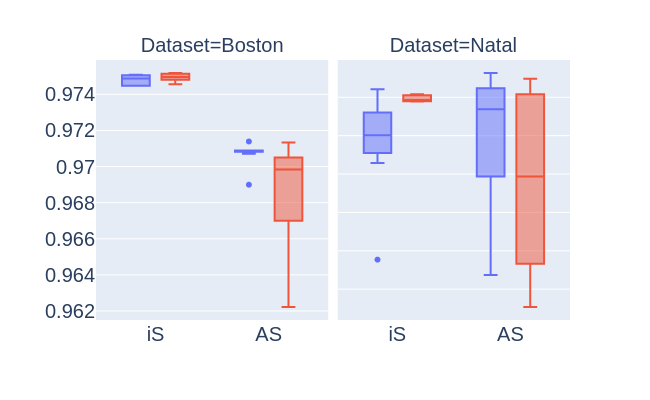
\includegraphics[width=0.8\linewidth, clip=true, trim=45px 50px 80px 30px]{img/ts-setups.png}
    \caption{R$^2$ comparison of \tinyisklearn and \autosklearn on TS datasets using different configuration setups. Blue: \textbf{regular}; red: \textbf{TM}.}
    \label{fig:ts-setups}
\end{figure}

As previously discussed, the best-performing AutoML tool for the \textbf{regular} setup varies as a function of the TS dataset considered. However, under the \textbf{TM} setup the pipelines from \isklearn outperform the ensembles from \autosklearn for all datasets.
%(even if \autosklearn has more cutoff timavailable for the evaluation). 
These results are explained by two factors. First, the performance of \isklearn pipelines is improved by the inclusion of more meta-folds, even if proportionally the cutoff time for the evaluation of each meta-fold is halved. Second, the performance of \autosklearn ensembles is reduced by the increase in cutoff time. One likely explanation is that the larger training time enables SMAC to select more complex ensembles, which tend to overfit in a time series setup using holdout.

To further investigate the impact of cutoff time and number of meta-folds, we extend our experimental design. Besides those factors, we also investigate the impact of increasing the total number of experiments \irace is allowed to perform. 
%  to comprise three experimental factors: 
%setups where we~(i)~reduce the chances that candidate evaluation is not completed within the cutoff time; (ii)~allow \irace to evaluate a larger number of candidate configurations, and/or; (iii)~assess our mid-level sampling generalization proposal, intended to provide the bottom-level sampling more data and thus reduce the chance for overfitting. 
% Our rationale is that CIFAR-10 was the most computationally demanding dataset in the previous section, and hence increasing the resources provided to \isklearn should lead to better-performing pipelines. 
%
%To accomplish these goals, we consider three experimental factors, namely 
%increased (i)~cutoff time, (ii)~configuration budget, and (iii)~number of meta-folds~($p$). 
Table~\ref{tab:exp-configs} depicts the setups we produce from these factors, where \textbf{regular} serves as baseline. With \textbf{20m}, \textbf{5k} and \textbf{TM 30m} we independently investigate increased (i)~cutoff time, (ii)~configuration budget, and (iii) number of meta-folds, respectively. In addition, since a total cutoff time of 30m may be impractical depending on the computational setup available, we investigate with \textbf{TM} and \textbf{TM 5k} whether halving the total cutoff time would be an option. For instance, the TS analysis above adopted \textbf{TM}, where halving the total cutoff time was compensated by the increased number of meta-folds.

% Setups dubbed \textbf{TM}~(short for \textit{triple meta-fold}) use $p=3$, i.e., the mid-level sampling procedure uses three meta-folds. Additionally, two setups allow increased configuration budget (\textbf{5k} and \textbf{TM 5k}), with 5000 experiments allowed instead of the previous 2000. Lastly, setups that consider increased cutoff time~(\textbf{20m} and \textbf{TM 30m}) allow for a doubled cutoff time w.r.t. their corresponding reference setups~(\textbf{regular} and \textbf{TM}, respectively).
% Complementarily, accuracy results for each setup~(columns) and dataset~(rows) are given in Table~\ref{tb:further-accuracy}. The best value obtained per benchmark among \isklearn pipelines is highlighted in boldface, and accuracies of ensembles from \autosklearn are also highlighted when they outperform all pipelines from \isklearn for the given benchmark. 

\begin{table}[!t]
\centering
\caption{Summary of the six configuration setups considered in this section. Regular~(\textbf{reg}.) stands for the configuration setup assessed in the previous section, used here as baseline.}
\label{tab:exp-configs}
\scalebox{0.85}{\begin{tabular}{r*{7}{c}}
\hline
\textbf{setup} & \textbf{reg.} & \textbf{20m} & \textbf{5k} & \textbf{TM 30m} & \textbf{TM} & \textbf{TM 5k}\\ \hline
\textbf{$p$} & 1 & 1 & 1 & 3 & 3 & 3 \\ \hline
\textbf{budget} & 2000 & 2000 & 5000 & 2000 & 2000 & 5000 \\ \hline
\textbf{cutoff} & 10m & 20m & 10m & 30m & 15m & 15m \\ \hline
\end{tabular}}
\end{table}

% When cutoff time was OK (Reuters), no experimental factor helped consistently, though more samples worsened performance slightly.
% CIFAR-10 results are outliers, likely because of the large gap to the state-of-the-art
% Increasing the number of experiments helps
% Increasing the number of samples helps, except for FMNIST where it is irrelevant
% Reducing cutoff time in general worsens performance, but the increased number of experiments helps, sometimes greatly FMNIST

% CT: if cutoff time was enough, doubling shouldn't affect greatly
% - Cutoff time was OK: Reuters
% - Cutoff time was not enough: CIFAR-10, FMNIST, SVHN, LMRD, AGNews
% 5k: if number of experiments was enough, increasing shouldn't affect greatly
% - Cutoff time was not enough, and more experiments didn't help: CIFAR-10
% - Cutoff time was not enough, but more experiments helped: FMNIST, SVHN, LMRD, AGNews
% TM: if number of samples was enough, tripling shouldn't affect greatly 
% - Cutoff time was not enough, and more samples didn't help: CIFAR-10, FMNIST
% - Cutoff time was not enough, but more samples helped: SVHN, AGNews

Boxplots given in Figure~\ref{fig:setups} depict accuracy scores for CV~(left column) and NLP~(right column) datasets, on which we focus due to the larger improvement margins observed in Section~\ref{sec:results}. However, margins as large as CIFAR-10 make results for this dataset outliers, and hence the following discussion focuses on the remaining ones. For a given plot, setups are ordered as in Table~\ref{tab:exp-configs}. We first remark that the differences in performance among setups is much more significant for CV datasets than for NLP ones. Apart from that, the most important factor observed was cutoff time, as only for Reuters we do not observe improvements under setup \textbf{20m}. For this dataset, none of the remaining factors consistently helped, though adopting more samples worsened performance slightly. For the remaining datasets, increasing either the number of experiments~(\textbf{5k}) or the number of meta-folds~(\textbf{TM}) improved performance. The only exception was FMNIST, for which increasing the number of meta-folds changed performance to a negligible rate. Finally, reducing the cutoff time did not compensate for the increased number of meta-folds~(\textbf{TM}), though the possibility of more experiments~(\textbf{TM 5k}) alleviated the loss in performance. Once again, FMNIST was an exception, since results under \textbf{TM 5k} were even better than for \textbf{TM 30m}.
% CIFAR-10 results are outliers, likely because of the large gap to the state-of-the-art
% Increasing the number of experiments helps
% Increasing the number of samples helps, except for FMNIST where it is irrelevant
% Reducing cutoff time in general worsens performance, but the increased number of experiments helps, sometimes greatly FMNIST

% For a given plot, setups are ordered as in Table~\ref{tab:exp-configs}. Results present interactions between application domain, dataset, and the experimental factors used to produce the setups we assess. Concerning application domain, the CV datasets seem to be more sensitive to configuration setup changes than the NLP ones. Furthermore, patterns are not consistent, even for datasets from the same domain. Still, we can observe overall that increasing configuration budget or cutoff time in single meta-fold setups mostly improves results. Similarly, the triple meta-fold approach can be useful, but often only if combined with increased configuration budget or cutoff time. This shows that while an increase in configuration budget or cutoff time is not necessary for experimental purposes, it might be desirable for certain applications.

\begin{figure}
    \centering
    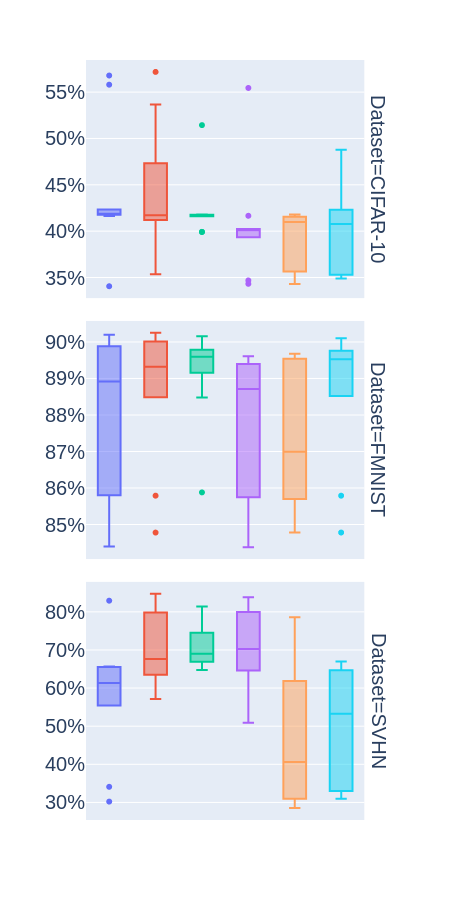
\includegraphics[width=0.49\linewidth, clip=true, trim=45px 70px 45px 60px]{img/cv-setups.png}
    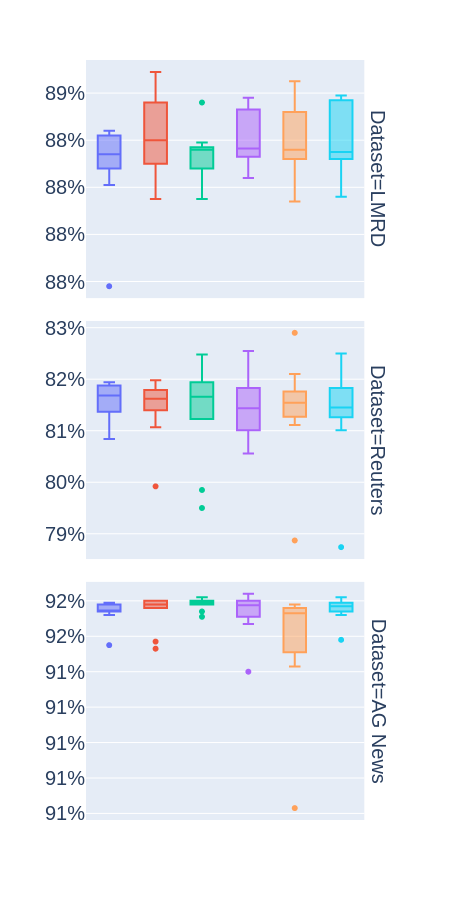
\includegraphics[width=0.49\linewidth, clip=true, trim=45px 70px 45px 60px]{img/nlp-setups.png}
    \caption{Accuracy comparison on CV~(left column) and NLP~(right column) datasets under alternative configuration setups. Within each plot, setups are ordered as in Table~\ref{tab:exp-configs}.}
    \label{fig:setups}
\end{figure}

% In general, 
% single meta-fold (SM) setups~(setups where the number of meta-folds $p=1$) are preferable to our previous approach~($p=3$). Do note that, while trends point to more favorable results with the single meta-fold approach, results about other factors are inconclusive. Specifically, increasing the number of experiments and/or the cutoff time does not necessarily lead to better results.
% Nonetheless, it is remarkable that changes to the configuration setup lead to a 42.32\% accuracy improvement on CIFAR-10 and to  21.73\% on SVHN. In fact, the improvement on CIFAR-10 leads to an accuracy higher than that of \autosklearn, which is also true for CIFAR-100. The most extreme situations concern FMNIST and SVHN, where performances are considerably different between pipelines from \isklearn and ensembles from \autosklearn. Further investigation on these datasets would be required to understand these significant gaps, but exceed the scope of this work. 

% \medskip
% Altogether, the experiments in this section have helped understand the impact of the different components of \isklearn. 
% Altogether, the experiments in this section indicate that the first configuration setup factor a practitioner should try to adjust is the cutoff time for a single experiment. If that is not feasible due to computational setup limitations, increasing the number of meta-folds can be an effective alternative, confirming the contribution of our generalized sampling.

% \begin{table}[]
% \centering
% \caption{Accuracy for each dataset/configuration setup pair. Ensembles produced by \autosklearn~(AS) are taken as baseline.}
% \label{tb:further-accuracy}
% \scalebox{0.78}{\begin{tabular}{r|*{6}{c}|cc}
% \hline
%  & \textbf{reg.} & \textbf{5k} & \textbf{30m} & \textbf{SM} & \textbf{SM 5k} & \textbf{SM 20m} & \textsc{AS} \\ \hline
% \textbf{C10} & 35.73 & 43.61 & 40.15 & \textbf{50.85} & 43.24 & 32.13 & 48.30 \\ \hline
% \textbf{C100} & 20.50 & 20.54 & 17.88 & 19.58 & 16.80 & \textbf{21.14} & 18.89 \\ \hline
% \textbf{FM} & 88.63 & 87.64 & 85.23 & 88.26 & 88.99 & \textbf{89.18} & \textbf{97.27} \\ \hline
% \textbf{SVHN} & 65.89 & 72.82 & 66.7 & 65.33 & \textbf{80.21} & 55.10 & 41.14\\ \hline
% \end{tabular}}
% \vspace{-12pt}
% \end{table}


% We next proceed to the pipeline composition assessment given in Table~\ref{tb:further-predictor}, where again rows depict benchmarks and columns the different experimental setups considered. Each cell lists the feature engineering~(\textsf{\footnotesize FE}) components (when used and, if so, in which order), and  predictors~(\textsf{\footnotesize Pred}) selected by \irace.
% Patterns in this table are much more clear. Concerning pre-processing, over two thirds of the cells include some FE component. Surprisingly, even if extraction is expected to be effective for computer vision problems, only half of the pipelines that include FE comprise extraction. More importantly, none of the pipelines that are best-performing for each benchmark use extraction. Among the best-performing pipelines, three out of four adopt feature selection, but differ as to how. 

% \begin{table}[!t]
% \centering
% \caption{Feature engineering (FE) and prediction (Pred) components selected for each dataset/configuration setup pair.}
% \label{tb:further-predictor}
% \scalebox{0.8}{\begin{tabular}{r*{8}{c}}
% \hline
% & & \textbf{reg.} & \textbf{5k} & \textbf{30m} & \textbf{SM} & \textbf{SM 5k} & \textbf{SM 20m}\\ \hline
% \multirow{2}{*}{\textbf{C10}} & \textsf{FE} & - & E & S\&E & \textbf{S} & E\&S & - \\
% & \textsf{Pred} & kNN & kNN & kNN & \textbf{SVM} & kNN & AB \\ \hline
% \multirow{2}{*}{\textbf{C100}} & \textsf{FE} & E & E\&S & - & - & S & \textbf{S} \\
% & \textsf{Pred} & kNN & kNN & DT & MLP & kNN & \textbf{MLP} \\ \hline
% \multirow{2}{*}{\textbf{FM}} & \textsf{FE} & S & - & S & E\&S & - & \textbf{-} \\
% & \textsf{Pred} & MLP & MLP & SVM & MLP & MLP & \textbf{MLP} \\ \hline
% \multirow{2}{*}{\textbf{SVHN}} & \textsf{FE} & S & S\&E & S & S & \textbf{S} & S \\
% & \textsf{Pred} & kNN & kNN & kNN & kNN & \textbf{SVM} & kNN \\ \hline
% \end{tabular}}
% \end{table}

% Regarding predictors, $k$-nearest neighbors~(kNN) is selected half of the times, although none of the best-performing pipelines are based on kNN. Yet, while this is a relatively simple prediction algorithm, most of the kNN-based pipelines use some of form of FE. Combined, these components lead to competitive performance on CIFAR-100 and Fashion MNIST w.r.t. the other pipelines. Out of the prediction algorithms that were in fact chosen in the best-performing pipelines, SVM and MLP are equally occurring. Altogether, these designs indicate that \isklearn balances the computational cost of its different components.
%The success of the latter might be correlated with the overall success of other more complex neural networks in computer vision problems. As for the former, SVMs had already been select on two out of three datasets of different domains, in our previous experiments.

